\section{Prueba 2: comunicaciones vehiculares en entornos urbanos}
En esta prueba se desea medir la calidad de las comunicaciones vehiculares en diferentes escenarios dentro de entornos urbanos. Durante esta prueba se desea medir más aspectos de la comunicación que en la prueba anterior: ruido de la comunicación, número de paquetes perdidos, tiempo que se tarda en enviar y recibir un paquete y \emph{delay} de las comunicaciones. Para ello se ha ampliado la aplicación de la prueba anterior para acceder a datos del módulo y hacer un mayor registro de \emph{logs}. Además, también se requería hacer la prueba con diferentes potencias de transmisión, y con una mayor o menor frecuencia de transmisión.

Se ha elegido como escenario de pruebas varias calles dentro de Bilbao, los escenarios seleccionados son los siguientes:
\begin{itemize}
	\item Envío de mensajes en intersecciones entre calles estrechas: se ha	realizado un recorrido entre las calles de Gran vía, Botica Vieja, el puente de Deusto y el puente Euskalduna.
	\item Envío de mensajes en calles altamente congestionadas: se ha realizado	en la Gran Vía y la calle Pozas.
	\item Envío de mensajes en vías de alta velocidad: se ha realizado un recorrido en la	autopista A-8. Se ha mantenido una distancia de entre 500 y 900 metros aproximadamente, para poder estimar la distancia en la que comienza a existir una perdida de paquetes.
\end{itemize}

\subsection{Resultados}
Las pruebas realizadas fueron satisfactorias. Las aplicaciones funcionaron correctamente, tan solo hubo un error en la aplicación al reiniciar una de las pruebas; el error pudo ser solucionado cerrando y volviendo a abrir la aplicación.

En la figura \ref{fig:prueba2-ui} se muestra la interfaz gráfica de la aplicación realizada con Python y Qt encargada de generar las estadísticas a partir de los datos obtenidos durante las pruebas.

\begin{figure}[H]
	\begin{center}
		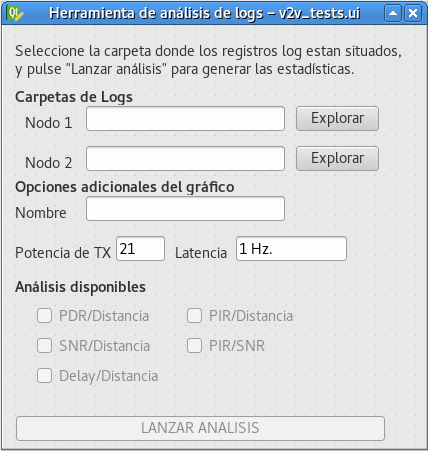
\includegraphics[scale=0.4]{prueba2-ui}
		\caption{Generador de gráficas}
		\label{fig:prueba2-ui}
	\end{center}
\end{figure}